\subsection{Automatic generation of test cases}
\label{sec-autotestcases}

A model, a statechart for instance, can also be used to specify certain scenarios and funcionalities relevant to the software. Considering that such model correct, is readable by a machine and its interpretation is well defined, one can use it to automatically generate functional test cases \cite{Maldonado:07}. This technique, in which test cases are automatically derived from a model, is called Model Based Test.

Since models are commonly based on finite state machines, the test cases in Model Based Test are often paths in the model. A path corresponds to a sequence of consecutive transitions. There are several ways to explore the model to obtain the paths. Depending on the complexity of the model and the exploration mode chosen, the number of test cases found will be huge. In fact, if one searches for all possible paths, the number of test cases will be infinite if the model contains cycles.

Hence, there are several criteria intended to guide the model exploration and generate the paths as test cases. Some of the them are described below and with further details in \cite{inpe10}:

\begin{itemize}

\item \textbf{All transitions}

A criterion that can be used to obtain test cases from statechart specifications. It requirers that every transition should be exercised at least once during testing.

\item \textbf{All simple paths}

Another criterion can be used with statecharts. Since all paths is an impossible achivement given the possibility that an infinite number of paths may exist, it is possible to requirer that every simple path in the model is exercised at least once during testing.

It is important to note that even though this two previous criteria seem similar to the ones described in~\ref{strucTest}, they are distinct. The ones described in this section are based on functional requirements and therefore constitute a kind of black-box test. The ones discribed in~\ref{strucTest} are based on the code implementation and are a type of white-box test.

\item \textbf{Distinguishing Sequence}

This criterion should be used for finite state machine models. Besides, the finite state machine must be deterministic, complete, strongly connected and minimal. 

First, a distinguishing sequence, SD, is searched. SD is an input sequence such that when applied to each state in the machine, the output produced is different, making it possible to identify the initial state to which SD was applied. The distinguishing sequence may not exist, in this case the criterion cannot be applied.

Second, for each transition $t$, an input sequence from the initial state up to including $t$ is generated. That sequence is called $\beta-sequence$.

We can then concatenate SD to end of each $\beta-sequence$ to obtain the test cases. When one of these test cases is executed, it will be specifically testing a transition and checking if this transition reached the expected state.

For the automaton in figure \ref{fig:automatonDS_UIO}, we have one possible SD = \textbf{B B}. In table \ref{tableDS} we have the complete set of $\beta-sequences$ to demonstrate the Distinguishing Sequence criterion.

\begin{figure}[htb]
\centering
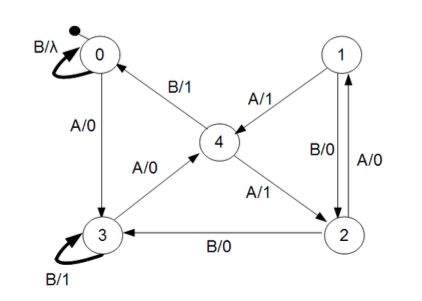
\includegraphics[width=7cm]{figuras/automatonDS_UIO}
\caption{\label{fig:automatonDS_UIO} Automaton extracted from \cite{inpe10}}
\end{figure}

\begin{table}
\begin{center}
\begin{tabular}{| l | l| l|}

\hline

$\beta-sequence$ & Transition & $\beta-sequence$ + SD \\ \hline

A & (0, 3) & A B B\\ \hline
B & (0, 0) & B B B\\ \hline
A A A A A & (1, 4) & A A A A A B B\\ \hline
A A A A B & (1, 2) & A A A A B B B\\ \hline
A A A A & (2, 1) & A A A A B B\\ \hline
A A A B & (2, 3) & A A A B B B\\ \hline
A A & (3, 4) & A A B B\\ \hline
A B & (3, 3) & A B B B\\ \hline
A A A & (4, 2) & A A A B B\\ \hline
A A B & (4, 0) & A A B B B\\
\hline
\end{tabular}
\end{center}
\caption{Distinguishing Sequence cases for automaton \ref{fig:automatonDS_UIO}. SD = "B B".\cite{inpe10}}
\label{tableDS}
\end{table}



\item \textbf{Unique Input-Output}

As mentioned in the previous criterion, the machine might not have a distinguishing sequence. In this case, it is still possible to identify each state based not only on the input, but on the output as well.

This criterion should be used for finite state machine models. Besides, the finite state machine must be deterministic, complete, strongly connected and minimal. 

First, for each state, an unique input-output sequence, UES, is searched. In each state, a breadth search is done and at every step, it is checked if the input and output is unique in comparison to the other states.

Second, a process to find $\beta-sequences$ is performed in the same way as the previous criterion.

Then, we can check to which state each final transition os the $\beta-sequences$ leads to by applying the UES sequences and observing their output.

For the automaton in \ref{fig:automatonDS_UIO}, table \ref{tableUES_1} shows the possible UES for each state. In table \ref{tableUES_2} we the whole set of $\beta-sequences$ and their concatenation with the respective UES. Both tables can be used to ilustrate the Unique Input-Output criterion.

\end{itemize}

\begin{table}
\begin{center}
\begin{tabular}{| l | l|}

\hline

State & UES \\ \hline

0 & B/$\lambda$\\ \hline
1 & A/1 A/1\\ \hline
2 & B/0\\ \hline
3 & B/1 B/1\\ \hline
4 & A/1 A/0\\

\hline
\end{tabular}
\end{center}
\caption{UES sequences for automaton \ref{fig:automatonDS_UIO}.\cite{inpe10}}
\label{tableUES_1}
\end{table}

\begin{table}
\begin{center}
\begin{tabular}{| l | l| l|}

\hline

$\beta-sequence$ & Transition & $\beta-sequence$ + UES \\ \hline

A & (0, 3) & A B B\\ \hline
B & (0, 0) & B B\\ \hline
A A A A A & (1, 4) & A A A A A A A\\ \hline
A A A A B & (1, 2) & A A A A B B \\ \hline
A A A A & (2, 1) & A A A A A A\\ \hline
A A A B & (2, 3) & A A A B B B\\ \hline
A A & (3, 4) & A A A A\\ \hline
A B & (3, 3) & A B B B\\ \hline
A A A & (4, 2) & A A A B \\ \hline
A A B & (4, 0) & A A B B \\
\hline
\end{tabular}
\end{center}
\caption{Unique Input-Output cases for automaton \ref{fig:automatonDS_UIO}.\cite{inpe10}}
\label{tableUES_2}
\end{table}



